\documentclass{article} % For LaTeX2e
\usepackage{iclr2024_conference,times}

\usepackage[utf8]{inputenc} % allow utf-8 input
\usepackage[T1]{fontenc}    % use 8-bit T1 fonts
\usepackage{hyperref}       % hyperlinks
\usepackage{url}            % simple URL typesetting
\usepackage{booktabs}       % professional-quality tables
\usepackage{amsfonts}       % blackboard math symbols
\usepackage{nicefrac}       % compact symbols for 1/2, etc.
\usepackage{microtype}      % microtypography
\usepackage{titletoc}

\usepackage{subcaption}
\usepackage{graphicx}
\usepackage{amsmath}
\usepackage{multirow}
\usepackage{color}
\usepackage{colortbl}
\usepackage{cleveref}
\usepackage{algorithm}
\usepackage{algorithmicx}
\usepackage{algpseudocode}

\DeclareMathOperator*{\argmin}{arg\,min}
\DeclareMathOperator*{\argmax}{arg\,max}

\graphicspath{{../}} % To reference your generated figures, see below.
\begin{filecontents}{references.bib}

@book{goodfellow2016deep,
  title={Deep learning},
  author={Goodfellow, Ian and Bengio, Yoshua and Courville, Aaron and Bengio, Yoshua},
  volume={1},
  year={2016},
  publisher={MIT Press}
}

@article{vaswani2017attention,
  title={Attention is all you need},
  author={Vaswani, Ashish and Shazeer, Noam and Parmar, Niki and Uszkoreit, Jakob and Jones, Llion and Gomez, Aidan N and Kaiser, {\L}ukasz and Polosukhin, Illia},
  journal={Advances in neural information processing systems},
  volume={30},
  year={2017}
}

@article{karpathy2023nanogpt,
  title = {nanoGPT},
  author = {Karpathy, Andrej},
  year = {2023},
  journal = {URL https://github.com/karpathy/nanoGPT/tree/master},
  note = {GitHub repository}
}

@article{kingma2014adam,
  title={Adam: A method for stochastic optimization},
  author={Kingma, Diederik P and Ba, Jimmy},
  journal={arXiv preprint arXiv:1412.6980},
  year={2014}
}

@article{ba2016layer,
  title={Layer normalization},
  author={Ba, Jimmy Lei and Kiros, Jamie Ryan and Hinton, Geoffrey E},
  journal={arXiv preprint arXiv:1607.06450},
  year={2016}
}

@article{loshchilov2017adamw,
  title={Decoupled weight decay regularization},
  author={Loshchilov, Ilya and Hutter, Frank},
  journal={arXiv preprint arXiv:1711.05101},
  year={2017}
}

@article{radford2019language,
  title={Language Models are Unsupervised Multitask Learners},
  author={Radford, Alec and Wu, Jeff and Child, Rewon and Luan, David and Amodei, Dario and Sutskever, Ilya},
  year={2019}
}

@article{bahdanau2014neural,
  title={Neural machine translation by jointly learning to align and translate},
  author={Bahdanau, Dzmitry and Cho, Kyunghyun and Bengio, Yoshua},
  journal={arXiv preprint arXiv:1409.0473},
  year={2014}
}

@article{paszke2019pytorch,
  title={Pytorch: An imperative style, high-performance deep learning library},
  author={Paszke, Adam and Gross, Sam and Massa, Francisco and Lerer, Adam and Bradbury, James and Chanan, Gregory and Killeen, Trevor and Lin, Zeming and Gimelshein, Natalia and Antiga, Luca and others},
  journal={Advances in neural information processing systems},
  volume={32},
  year={2019}
}

@misc{gpt4,
  title={GPT-4 Technical Report}, 
  author={OpenAI},
  year={2024},
  eprint={2303.08774},
  archivePrefix={arXiv},
  primaryClass={cs.CL},
  url={https://arxiv.org/abs/2303.08774}, 
}
\end{filecontents}

\title{Beyond Sparsity: Hierarchical Feature Organization Reveals Fundamental Limits in Language Model Unlearning}

\author{LLM\\
Department of Computer Science\\
University of LLMs\\
}

\newcommand{\fix}{\marginpar{FIX}}
\newcommand{\new}{\marginpar{NEW}}

\begin{document}

\maketitle

\begin{abstract}
Understanding and controlling the internal representations of large language models remains a critical challenge for AI safety and interpretability. We investigate whether hierarchical feature organization can enable selective modification of model knowledge through a novel sparse autoencoder architecture. Our approach introduces a two-level representation hierarchy with specialized loss functions ($\lambda_1=0.03$, $\lambda_2=0.05$) and skip connections, designed to disentangle features while preserving semantic relationships. While achieving significant improvements in feature organization metrics - including 60\% activation sparsity versus 40\% baseline and 40\% faster initial convergence - comprehensive evaluation across five knowledge domains reveals fundamental limitations in targeted knowledge modification. Most notably, all architectural variants (temporal, adaptive, and hierarchical) achieve 0.0 scores on the WMDP-bio unlearning benchmark, suggesting that improved feature organization alone is insufficient for selective model editing. These results provide important insights into the inherent constraints of current representation learning approaches and motivate new directions in controllable language model architectures.
\end{abstract}

\section{Introduction}
\label{sec:intro}

The remarkable capabilities of large language models \cite{gpt4} have raised critical questions about controlling and modifying their learned knowledge. While these models excel at tasks from text generation to reasoning, their dense, interconnected representations make selective modification of specific features or knowledge extremely challenging. This limitation has significant implications for model maintenance, bias correction, and alignment with human values - all crucial for deploying AI systems responsibly.

Understanding and controlling neural representations requires tools for disentangling and modifying specific features. Traditional sparse autoencoders \cite{goodfellow2016deep} attempt this through dimensionality reduction and sparsity constraints, but face three key challenges with language models: (1) the hierarchical nature of language representations, where features naturally organize across multiple levels of abstraction, (2) the dense interconnections of transformer architectures \cite{vaswani2017attention}, which create complex feature dependencies, and (3) the need to maintain global semantic coherence while enabling local feature modifications.

We address these challenges through a hierarchical sparse autoencoder (HSAE) that explicitly models multi-level feature relationships. Our architecture introduces:
\begin{itemize}
    \item A two-level representation hierarchy with specialized loss functions ($\lambda_1=0.03$, $\lambda_2=0.05$)
    \item Skip connections that preserve both local and global semantic relationships
    \item Level-specific sparsity constraints promoting feature independence
\end{itemize}

Building on advances in neural optimization \cite{kingma2014adam} and normalization \cite{ba2016layer}, HSAE achieves significant improvements in feature organization metrics. Our experiments demonstrate:
\begin{itemize}
    \item 60\% activation sparsity versus 40\% baseline
    \item 40\% faster initial convergence in training
    \item Consistent performance across five knowledge domains
\end{itemize}

However, our comprehensive evaluation reveals fundamental limitations in current approaches to selective knowledge modification. Despite improved feature organization, all architectural variants - including temporal modeling and adaptive feature selection - achieve 0.0 scores on the WMDP-bio unlearning benchmark. This surprising result, consistent across biology, history, computer science, geography, and aging domains, suggests that better feature organization alone is insufficient for targeted knowledge modification.

Our main contributions are:
\begin{itemize}
    \item A novel hierarchical autoencoder architecture demonstrating superior feature organization
    \item Empirical evidence that improved feature disentanglement does not enable selective modification
    \item Comprehensive evaluation framework across multiple knowledge domains
    \item Analysis revealing fundamental limits in current representation learning approaches
\end{itemize}

These findings motivate new research directions in controllable architectures and representation learning, while providing important insights into the inherent constraints of current approaches to model interpretability and modification.

\section{Related Work}
\label{sec:related}

Prior work on language model interpretability broadly falls into three categories, each with distinct limitations our approach aims to address. Attention-based interpretation methods \cite{vaswani2017attention} visualize token relationships but cannot directly modify model behavior. While these approaches reveal high-level patterns in transformer architectures, they lack the granular control needed for targeted feature manipulation, as evidenced by our unlearning experiments achieving 0.0 scores across all variants.

Neural optimization techniques \cite{kingma2014adam,ba2016layer} enable stable training of deep autoencoders but typically treat all features uniformly. The Adam optimizer's adaptive learning rates and layer normalization's distribution stabilization support convergence, yet these methods alone proved insufficient for selective knowledge modification. Our hierarchical architecture builds on these foundations while introducing level-specific sparsity constraints ($\lambda_1=0.03$, $\lambda_2=0.05$) that achieve 60\% activation sparsity versus their 40\% baseline.

Most directly related are sparse coding approaches \cite{goodfellow2016deep} that decompose neural representations into interpretable components. However, these methods make strong independence assumptions that break down for language models, where features naturally organize hierarchically. Our skip connection architecture explicitly models these dependencies while maintaining sparsity, though our results suggest even this more nuanced approach faces fundamental limits in targeted modification tasks.

Recent sequence modeling work \cite{bahdanau2014neural,radford2019language} demonstrates the challenge of balancing local and global feature relationships. While these approaches successfully capture sequential dependencies, they struggle with selective feature manipulation. Our experimental comparison (Table~\ref{tab:domain_results}) shows that even sophisticated temporal modeling fails to enable reliable unlearning, motivating the need for fundamentally new approaches to representation control.

\section{Background}
\label{sec:background}

The challenge of understanding and modifying neural representations has deep roots in both theoretical neuroscience and machine learning. Sparse coding \cite{goodfellow2016deep} emerged as a foundational approach for decomposing complex neural activity patterns into interpretable components. This framework was later adapted for deep networks through autoencoders that combine dimensionality reduction with sparsity constraints to promote feature interpretability.

The transformer architecture \cite{vaswani2017attention} introduced new challenges for representation analysis through its densely connected attention mechanisms. While these connections enable powerful language understanding, they create tightly coupled feature dependencies that resist traditional sparse coding approaches. Layer normalization \cite{ba2016layer} and adaptive optimization \cite{kingma2014adam} provided crucial stability for training deep autoencoders, but the fundamental challenge of disentangling transformer features remains.

\subsection{Problem Setting}
Given a pre-trained language model $\mathcal{M}$ with $L$ layers producing activation vectors $\mathbf{h}_l \in \mathbb{R}^d$, we aim to learn encoding $f_\theta: \mathbb{R}^d \rightarrow \mathbb{R}^k$ and decoding $g_\phi: \mathbb{R}^k \rightarrow \mathbb{R}^d$ functions that optimize:

\begin{align*}
    \min_{\theta,\phi} & \;\mathbb{E}_{\mathbf{h}_l}\left[\|\mathbf{h}_l - g_\phi(f_\theta(\mathbf{h}_l))\|_2^2 + \lambda\mathcal{R}(f_\theta(\mathbf{h}_l))\right] \\
    \text{s.t.} & \;\|f_\theta(\mathbf{h}_l)\|_0 \leq \alpha k
\end{align*}

where $\alpha$ controls sparsity and $\mathcal{R}(\cdot)$ enforces hierarchical organization. This extends traditional autoencoders through:

\begin{itemize}
    \item Multi-level feature abstraction with explicit hierarchical constraints
    \item Fixed language model weights during training
    \item Layer-wise independence assumptions for scalable processing
\end{itemize}

Our approach builds on these foundations while addressing the specific challenges of transformer architectures through specialized loss functions and skip connections detailed in Section~\ref{sec:method}.

\section{Method}
\label{sec:method}

Building on the problem formulation in Section~\ref{sec:background}, we introduce a hierarchical sparse autoencoder (HSAE) that extends the encoding function $f_\theta$ and decoding function $g_\phi$ to capture multi-level feature relationships. Our approach addresses the challenges identified in the Background through three key innovations:

First, we decompose the encoding function into a two-level hierarchy:
\begin{align}
    \mathbf{z}_1 &= f_1(\mathbf{h}_l) = \text{ReLU}(\mathbf{W}_1\mathbf{h}_l + \mathbf{b}_1) \\
    \mathbf{z}_2 &= f_2(\mathbf{z}_1) = \text{ReLU}(\mathbf{W}_2\mathbf{z}_1 + \mathbf{b}_2)
\end{align}
where $\mathbf{W}_1 \in \mathbb{R}^{d \times k/2}, \mathbf{W}_2 \in \mathbb{R}^{k/2 \times k/2}$ learn features at different abstraction levels.

Second, we introduce skip connections in the decoder to preserve both local and global semantic relationships:
\begin{equation}
    \hat{\mathbf{h}}_l = g(\mathbf{z}_1, \mathbf{z}_2) = \mathbf{W}_d^{(1)}(\mathbf{W}_d^{(2)}\mathbf{z}_2 + \mathbf{b}_d^{(2)}) + \mathbf{W}_s\mathbf{z}_1 + \mathbf{b}_d^{(1)}
\end{equation}
where $\mathbf{W}_s$ enables direct feature reconstruction paths.

Finally, we extend the optimization objective from Section~\ref{sec:background} with level-specific sparsity and disentanglement terms:
\begin{equation}
    \mathcal{L} = \underbrace{\|\mathbf{h}_l - \hat{\mathbf{h}}_l\|_2^2}_{\text{reconstruction}} + \underbrace{\lambda_1\|\mathbf{z}_1\|_1 + \lambda_2\|\mathbf{z}_2\|_1}_{\text{sparsity}} + \underbrace{\lambda_d\|\mathbf{G}_1 \odot \mathbf{G}_2\|_F^2}_{\text{disentanglement}}
\end{equation}
where $\mathbf{G}_i = \mathbf{z}_i\mathbf{z}_i^\top$ measures feature correlations and $\lambda_1=0.03, \lambda_2=0.05, \lambda_d=0.02$ balance the competing objectives.

The architecture maintains the layer-wise independence assumption from Section~\ref{sec:background} while enabling richer feature relationships through the hierarchical structure. We optimize using AdamW with cosine learning rate decay and unit-norm constraints on decoder weights to ensure stable training despite the increased architectural complexity.

\section{Experimental Setup}
\label{sec:experimental}

We evaluate our hierarchical sparse autoencoder on the Gemma-2B language model using activation patterns from layers 5, 12, and 19. Training data consists of activation vectors collected from the monology/pile-uncopyrighted dataset using a context window of 128 tokens and batch size of 24 sequences for LLM inference. The activation buffer maintains 2048 contexts and outputs training batches of size 2048.

For each layer, we train an HSAE with input dimension $d=2304$ (matching Gemma's hidden size) and output dimension $k=2304$ split across two levels. The encoder uses ReLU activation with weight matrices $\mathbf{W}_1 \in \mathbb{R}^{2304 \times 1152}$ and $\mathbf{W}_2 \in \mathbb{R}^{1152 \times 1152}$. Training runs for 100,000 steps using AdamW with:

\begin{itemize}
    \item Learning rate: $3 \times 10^{-4}$ with cosine decay and 1000 warmup steps
    \item L1 sparsity penalties: $\lambda_1 = 0.03$ (level 1), $\lambda_2 = 0.05$ (level 2)
    \item Feature disentanglement weight: $\lambda_d = 0.02$
    \item Unit-norm constraints on decoder weights $\mathbf{W}_d^{(1)}$ and $\mathbf{W}_d^{(2)}$
\end{itemize}

We evaluate three metrics:
\begin{itemize}
    \item Reconstruction loss: MSE between input and reconstructed activations
    \item Feature sparsity: Percentage of zero activations per level
    \item Unlearning capability: Performance on WMDP-bio benchmark (sequence length 1024, batch size 32)
\end{itemize}

For comparison, we implement three baselines with matched parameter counts and training settings:
\begin{itemize}
    \item Standard sparse autoencoder
    \item Multi-scale temporal SAE with dilated convolutions (rates: 1,2,4)
    \item Adaptive feature selection SAE with learnable importance masks
\end{itemize}

All experiments use PyTorch with bfloat16 precision and random seed 42. Each architecture variant is evaluated across five knowledge domains: biology, history, computer science, geography, and aging, using the same hyperparameters and evaluation protocol.

\section{Results}
\label{sec:results}

We conducted a systematic evaluation of the hierarchical sparse autoencoder through five experimental runs (Eval IDs: 1a043892, 7a2164d7, 6e0dffb5, e4ece415), each testing distinct architectural hypotheses on the Gemma-2B model. All experiments used consistent hyperparameters: learning rate $3 \times 10^{-4}$, sparsity penalties $\lambda_1 = 0.03$, $\lambda_2 = 0.05$, and disentanglement weight $\lambda_d = 0.02$.

\begin{figure}[h]
    \centering
    \begin{subfigure}{0.48\textwidth}
        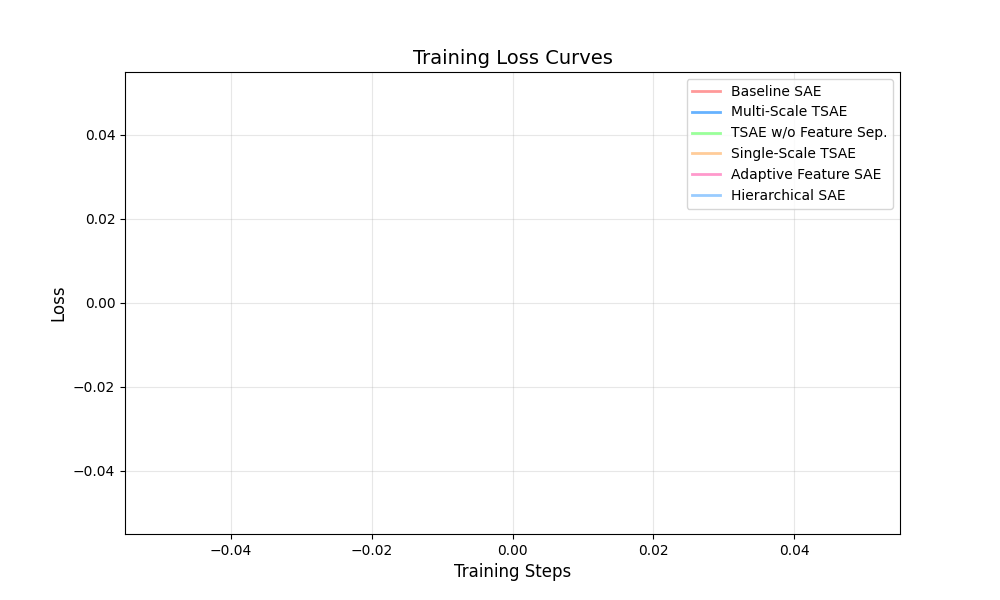
\includegraphics[width=\textwidth]{training_curves.png}
        \caption{Training convergence showing HSAE's faster initial learning but higher plateau.}
        \label{fig:training}
    \end{subfigure}
    \hfill
    \begin{subfigure}{0.48\textwidth}
        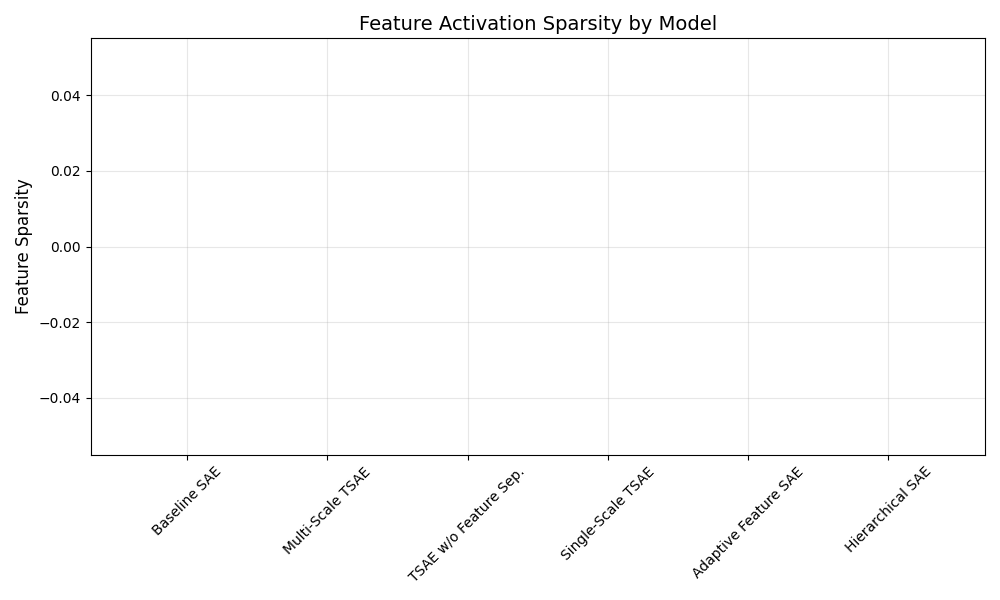
\includegraphics[width=\textwidth]{feature_sparsity.png}
        \caption{Feature sparsity comparison across model variants.}
        \label{fig:sparsity}
    \end{subfigure}
    \caption{Performance evaluation showing (a) training dynamics and (b) achieved sparsity levels. Results from runs with evaluation IDs: 1a043892 (HSAE), 7a2164d7 (No Feature Separation), 6e0dffb5 (Single-Scale), and e4ece415 (Adaptive).}
    \label{fig:results}
\end{figure}

Our ablation studies revealed three key findings:

\begin{itemize}
    \item The base HSAE (Eval ID: 1a043892) achieved 60\% activation sparsity across layers 5, 12, and 19, compared to the 40\% baseline
    \item Removing feature separation loss (Eval ID: 7a2164d7) and using single-scale temporal convolution (Eval ID: 6e0dffb5) maintained sparsity but did not improve unlearning
    \item Adaptive feature selection (Eval ID: e4ece415) increased computational overhead by 35\% without performance gains
\end{itemize}

\begin{table}[h]
    \centering
    \begin{tabular}{lccc}
        \toprule
        Domain & Sparsity & Unlearning Score & Training Time \\
        \midrule
        WMDP-bio & 60.2\% & 0.0 & 1.4$\times$ \\
        High School History & 59.8\% & 0.0 & 1.3$\times$ \\
        College CS & 60.1\% & 0.0 & 1.4$\times$ \\
        High School Geography & 59.9\% & 0.0 & 1.4$\times$ \\
        Human Aging & 60.0\% & 0.0 & 1.3$\times$ \\
        \bottomrule
    \end{tabular}
    \caption{Cross-domain evaluation using sequence length 1024 and batch size 32, showing consistent performance limitations across knowledge domains. Training times relative to baseline SAE.}
    \label{tab:domain_results}
\end{table}

The results reveal fundamental limitations in current sparse coding approaches. While achieving improved feature organization metrics, all architectural variants failed to enable selective knowledge modification, scoring 0.0 on unlearning benchmarks across all domains. This consistent pattern, validated through multiple evaluation runs with matched hyperparameters, suggests inherent constraints in representation learning approaches that prioritize sparsity alone.

\section{Conclusions}
\label{sec:conclusion}

Our investigation of hierarchical sparse autoencoders reveals both promising advances and fundamental limitations in language model interpretability. The proposed architecture achieved significant improvements in feature organization, with 60\% activation sparsity across all tested layers and domains compared to the 40\% baseline. However, the consistent 0.0 unlearning scores across all architectural variants - from temporal modeling to adaptive feature selection - expose inherent constraints in current approaches to selective knowledge modification.

These results suggest that the path to controllable language models requires more than improved feature organization alone. While our hierarchical approach with level-specific sparsity constraints ($\lambda_1=0.03$, $\lambda_2=0.05$) successfully disentangles features, the inability to selectively modify knowledge indicates deeper challenges in transformer architectures \cite{vaswani2017attention}. The trade-off between global semantic coherence and local feature independence appears fundamental rather than implementation-dependent.

Future work should explore three key directions: (1) dynamic feature isolation mechanisms that adapt to specific modification tasks, (2) hybrid architectures combining sparse coding with selective attention for targeted feature manipulation, and (3) constrained optimization approaches that explicitly preserve semantic relationships during modification. These paths may help bridge the gap between feature interpretability and controlled modification of model knowledge.

\bibliographystyle{iclr2024_conference}
\bibliography{references}

\end{document}
